\section{Background}
We provide a brief review of symbolic execution and describe the key features
of a hardware design that necessitate a new approach for symbolic execution. We
explain the recursive strategy for symbolic execution and provide a brief
overview of the Coq proof assistant.

\subsection{Symbolic Execution}
In symbolic execution formal parameters to a program's entry point are
assigned symbolic values. The program is then simulated by a symbolic execution
engine that uses the symbolic values in place of concrete literals. As
execution continues the resulting symbolic expressions propagate throughout the program's
state.

In addition the symbolic state, the symbolic execution engine keeps track
of the \emph{path condition} (\pathcondition) for the current path of execution. When execution begins the path condition is initialized
to \texttrue. At each conditional branch the condition $c$ is evaluated. If $\pathcondition
\rightarrow c$ is valid, the $\mathtt{then}$ branch is taken and the path constraint is
updated, $\pathcondition := \pathcondition \wedge c$. If $\pathcondition \rightarrow \neg c$ is valid, the $\mathtt{else}$
branch is taken and the path constraint is updated, $\pathcondition := \pathcondition \wedge \neg
c$. If neither $\pathcondition \rightarrow c$ nor $\pathcondition \rightarrow \neg c$ hold, then both
branches are possible. Execution forks and both branches are explored in turn
with the path condition updated appropriately for each branch.

All the paths explored through the program form a logical tree \tree. The root represents the
program's entry point and each node of the
tree represents a line of code in the program. Associated with each node is the
(partially) symbolic state of the program and the path condition at that point
of execution. A path in the tree from root to leaf
represents a path of execution through the program.

\ab{Figures not captioned or labeled.}


Figure~\ref{fig:se} demonstrates the idea. 
For example, for the code in
Figure~\ref{fig:sea}, if $\mathtt{reset}$ and $\mathtt{count}$ are initialized
with the symbolic values $r_0$ and $c_0$, respectively, then after symbolically
executing lines 1, 3, and 4 count may be set to the symbolic expression $c_0 +
1$ as shown in Figure~\ref{fig:sec}. In addition to the (partially) symbolic
state that is maintained, a symbolic execution engine keeps track of the
\emph{path condition}. The path condition is a conjunction of propositions that
accrue at each conditional branch point in the program. There is one path
condition per path of execution through the code. In Figure~\ref{fig:sec} the
path condition for the path through lines 1, 3, 4, 5, 6 is shown. When execution
reaches the $\mathtt{ERROR}$ at line 6 the path condition is $\mathit{pc} := r_0
== 0 \wedge c_0 + 1 > 3$. This expression can then be solved using a standard,
off-the-shelf SMT solver to find a satisfying solution, say $r_0 := 0$ and $c_0
:= 3$. Substituting these values for $\mathtt{reset}$ and $\mathtt{count}$,
respectively and executing the code concretely could cause execution to follow
the same path as was followed symbolically.

\begin{figure}
  \centering
  \begin{subfigure}[b]{0.3\textwidth}
    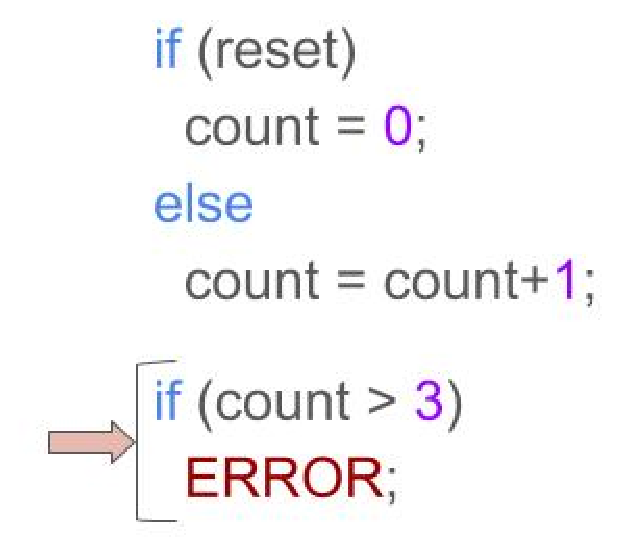
\includegraphics[width=\textwidth]{secode}
    \caption{Caption}
    \label{fig:sthg}
    \end{subfigure}
  \quad
  \begin{subfigure}[b]{0.3\textwidth}
    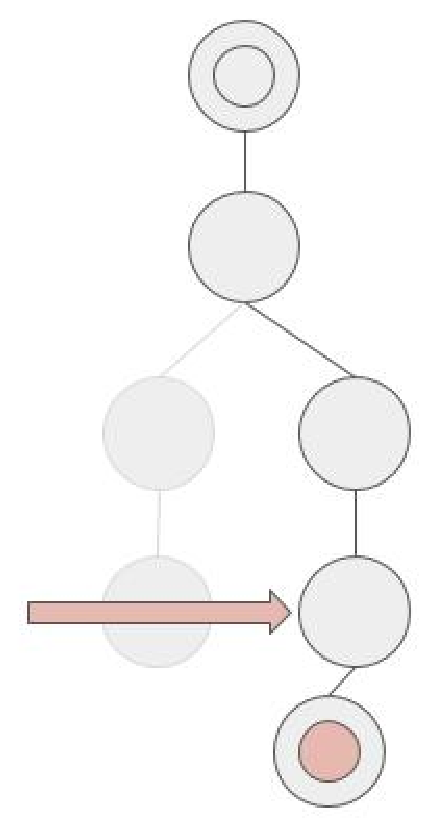
\includegraphics[height=2in]{setree}
    \caption{Caption}
    \label{fig:sthg}
    \end{subfigure}
  \quad
  \begin{subfigure}[b]{0.3\textwidth}
    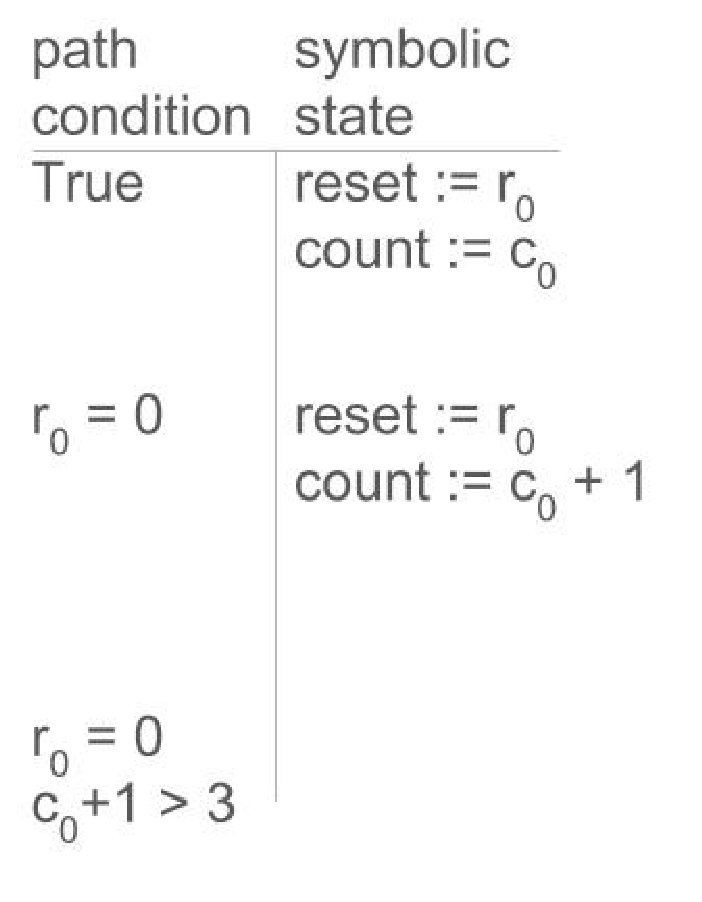
\includegraphics[height=2in]{setable}
    \caption{Caption}
    \label{fig:sthg}
    \end{subfigure}
  \caption{Global Caption}
  \label{Globallabel}
  \end{figure}
  
\subsection{Register Transfer Level Hardware Designs}
\cks{Quick explanation of challenges of HW designs and how Zhang et al. convert
  HW to SW for the symbolic execution.}


\subsection{Recursive Search Strategy for Symbolic Execution}
\cks{English description of strategy and three properties}

The symbolic execution engine
maintains the current, partially symbolic state of the program and the current
\emph{path condition}. The path condition is a conjunction of propositions over
input and state variables that define the path through the program code taken to
reach the current state.


\cks{Brain dump a bunch of mostly terrible text to get started.}
We model the processor as a vector $R$ of state registers $R = <r_0, r_1,
\ldots, r_n>$. At each step of execution (clock cycle) the valuation of each
register may change. New state is determined by the Boolean and bitvector
arithmetic combination of current state plus input values. $\forall m, r'_m =
\delta(R,I)$.

In concrete execution registers hold concrete values $(v_0, v_1, \ldots, v_n)$
at each clock cycle. In symbolic execution the concrete values are replaced with
symbolic values $(\phi_0, \phi_1, \ldots, \phi_n)$ and so are input values.
As execution continues, symbolic values propagate through the design.

The symbolic state is modeled as a tuple $\psi := (S,\pi)$ where $S$ is the
vector of registers containing a combination of symbolic and concrete state $S
:= <s_0, s_1, \ldots, s_n>$. As execution continues, symbolic values propagate
through the design.

The recursive symbolic execution strategy utilizes two instantiation operations. 
They define them in the following way: 

``Let $\mathcal{E}$ represent the symbolic exploration of one clock cycle of a processor modeled by $M$. Let $n_r = (s_r,\pi_r)$ be the root node of tree $\mathcal{E}$ and let $n_l = (s_l,\pi_l)$ be a leaf node of the same tree. 
Then $s_r \circ \pi_l$ represents the set of concrete states, and $s_l \circ \pi_l$ represents the set of concrete next-states, that are at the end-points of the path from $n_r$ to $n_l$.'' \cite{zhang2018recursive}

For our proof we let $\mathtt{concretize\_root}=  s_r \circ \pi_l$ and $\mathtt{concretize\_leaf} =  s_l \circ \pi_l$.





\subsection{Using Coq as a Verification Tool}

Coq is a formal, interactive proof assistant that allows for machine-checked proofs of systems. 
It implements the inductive language Gallina, which is based on the \textit{Calculus of Inductive Constructions}, a typed $\lambda$-calculus. It allows definitions of methods that can be evaluated, the expression of theorems and software specifications, and assists the user in building machine-checkable proofs. If the proof is complete, it will compile.


%There are four main structures in Coq that we use in our proof:
%\begin{itemize}
%\item \emph{Axiom} is used to express properties that do not need to be proven. These are meant to be accepted as ground truth in the system. 
%\item \emph{Definition} and \emph{Fixpoint} are used to define methods.
%\item \emph{Variable} defines local variables.
%\item \emph{Theorem} expresses a property that needs to be proven.
%\end{itemize}

 

Additionally, we make use of Coq's module system, representing different parts of our system as modules.  There is a module defining concrete execution, a module defining symbolic execution that includes the King properties as axioms, and a module defining the recursive symbolic execution strategy that includes the requirements laid out by Zhang et al. as axioms and the correctness property expressed as a theorem.

Our definitions and fixpoints are the methods that are implemented
in the system, such as execution of the list of trees provided by the recursive
symbolic execution tool. Our variables are system-specific variables, such as the
initial state and the error states, and they are contained in the backwards symbolic execution module as well.

We utilize the built-in ``logic'' library for assistance in small proofs and the ``ensembles'' library for assistance reasoning about finite sets. Additionally, we use the built-in ``list'' structure to represent lists of symbolic execution trees.









